\documentclass{article}
\usepackage{amsmath}
\usepackage{amssymb}
\usepackage[compact]{titlesec}
\usepackage{graphicx}
\usepackage{tikz}
\usetikzlibrary{calc,fadings,decorations.pathreplacing,shapes,shapes.multipart,arrows,shapes.misc,intersections,positioning}
\usepackage{wrapfig}
\usepackage{bm}
\usepackage[autostyle, english = american]{csquotes}
\MakeOuterQuote{"}
\graphicspath{{./}}

\newcommand{\cf}{\textit{cf.} }
\newcommand{\ie}{\textit{i.e.} } 
\newcommand{\eg}{\textit{e.g.} }
\newcommand{\vs}{\textit{vs.} } 
\newcommand{\etal}{\textit{et al.} }
\newcommand{\etc}{\textit{etc.} }
\newcommand{\rev}[1]{{\color{red}#1}}

\newcommand{\up}{\mathord{\uparrow}}
\newcommand{\dn}{\mathord{\downarrow}}
\newcommand{\I}{\mathbb{I}}

\renewcommand{\vec}[1]{\boldsymbol{\mathbf{#1}}}
\newcommand{\qed}[0]{$\blacksquare$}

\newcommand{\reply}[1]{{\color{black}#1}}

\textwidth = 6.5 in
\textheight = 9 in
\oddsidemargin = 0.0 in
\evensidemargin = 0.0 in
\topmargin = 0.0 in
\headheight = 0.0 in
\headsep = 0.0 in
\parskip = 0.2in
\parindent = 0.0in

% \definecolor{darkblue}{rgb}{0.1,0.2,0.6} \definecolor{darkred}{rgb}{0.8,0.1,0.2}
% \usepackage[colorlinks,citecolor=darkblue,linkcolor=darkred,urlcolor=darkblue]{hyperref}

\begin{document}
\large

{\bf Reply to the First Referee -- BF13677/Zhou}

\color{blue}

The authors investigate a quench problem where two critical bosonic chains are initially separated and then coupled by a conformal defect. This generalizes earlier treatments, where the chains were simply connected. They determine the fidelity (the negative logarithm of the overlap of the initial and the final ground state for chain lengths L) and the Loschmidt echo (the negative logarithmic overlap of the evolved state after some time t with the initial ground state). Since these overlaps decay as power laws, the logarithms vary as lnL and lnt, respectively. For a simple connection of the chains, the prefactors are known to be 1/8 and 1/4, respectively. For a defect, the authors find, that they can vary continuously with the defect transmission, depending on the boundary conditions at the chain ends and at the defect. This is derived analytically via a path- integral picture of the two quantities and conformal mappings. It is also verified by numerical calculations on oscillator chains, based on explicit expressions of the ground states in terms of boson operators from which the overlaps can be obtained as determinants.

Given that such varying exponents have a long history and were found also for the entanglement entropy in chains with defects, this is an interesting topic and the results are worth publishing. However, there are a couple of points to be clarified or changed.

\reply{We first acknowledge the effort of this respectful referee to read our manuscript thoroughly and provide constructive comments. We will address the issues below.}

(1) In order to obtain the correct result for the known case, the authors have to add a constant beta/12 in (21). However, the derivation in Appendix A is not right. The relation (A5) between the Hamiltonians in the staircase and in the strip differs by a sign from the one given in Ref. [32]. I think that the argument must be different. Usually, the universal terms in free energies are determined via appropriate non-conformal transformations which bring in the energy- momentum tensor. In this context one wonders about additional constants coming from the starting states in the path integral representation.

\begin{figure}[h]
\centering
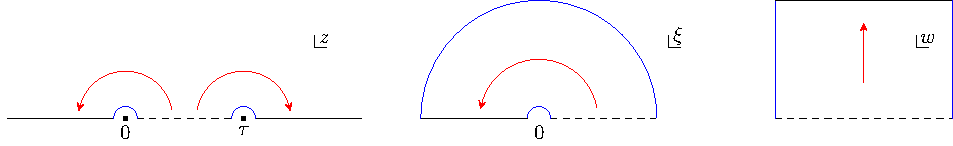
\includegraphics[width=\columnwidth]{/images/fig_H-tau_fold.pdf}
\caption{Conformal transformation from the slit to cylinder.}
\label{fig:H-tau_fold}
\end{figure}

\reply{
We thank the referee for pointing out this sign error, in fact we used the $w \rightarrow \xi \rightarrow z$ order in the calculation as opposed to the $z \rightarrow \xi \rightarrow w$ order of the conformal transformation in the figure. We have fixed them.  

Nevertheless we hold our opinion of using these two corrections to account for the missing $\frac{1}{12}\beta$. Let us reiterate our arguments. 

The first correction comes from mapping the slit diagram to the annulus (in Fig. 6).  Before doing this conformal transformation, the short distance regulator is small on the $z$ plane. Hence the contribution of the free energy coming from introducing the two blue lines are small. However, after the transformation, we implicitly choose another regulator which is small on the $\xi$ plane. But by the change of this short distance cutoff, the $\xi$ plane erroneously contribute a $- \frac{c}{6} \ln \frac{r_2}{r_1}$ term from the outer surface. The compensation $+\frac{c}{6} \ln \frac{r_2}{r_1} = \frac{c}{6}\beta$ is the correction we are talking about. 

The is the lesson we learned from the Cardy-Peschel paper, where there are two explicit examples of computing the free energies of a corner and a cone. Both objects should be regarded as infinitely extended without boundaries at certain radii. The authors computed the correct results by conformally mapping the geometry to whole plane (or upper half plane) and contrasted with the calculation of the truncated corner and cone with both short and long distance regulators. They found that the discrepancies of the truncated cone and corner w.r.t. to the correct results come from the outer boundary contribution. By subtracting this otherwise nonexistent contribution using their proposed geodesic curvature formula, they are able to recover the correct result. We believe that the mapping from the $z$ to $\xi$ plane result in the same situation here. 

We also change Fig 5, where in the left panel there is no vertical line IR regulator. So after doing the $\exp$ conformal transformation, the center diagram should be the upper half plane minus the small circle around $\xi = 1$. This is also an extended object, much the same way as the cone and corner in the Cardy-Peschel paper. To evaluate this extended diagram, we manually add another big semi-circle centered at $\xi = 1$ with radius $R_{\xi } \gg 1$. This will introduce a $-\frac{c}{6} \beta $ term that should not be there. So in both cases we should compensate $+\frac{c}{6}\beta$. 

Then we move on to the $\xi$ to $w$ plane transformation. The staircase geometry Hamiltonian and the plane Hamiltonian is differed by the Schwartzian term in the transformation rule of the stress tensor, which gives $-\frac{c}{12} \beta $ correction. By gathering the two terms, we do get the desired $\frac{c}{12}\beta$ correction. 

The content of this reply is supplemented in App. C. We request the referee to reconsider the presented arguments.
}

(2) I also find the whole presentation of the mapping unsatisfactory. In part, this has to with the fact that no lengths are indicated in the figures.

For the fidelity, one maps in Fig. 5 the initial strip to an annulus with inner and outer radii determined by the length of the strip which goes to infinity. Then one moves the point, where the boundary condition changes, to the origin, which means that, in the strip, it is moved to the far left and disappears there. I cannot see, how the calculation then proceeds. In [25], a different conformal map was used.

\reply{
We have added more descriptions in the text around Fig.5 and Fig.6 about the conformal mappings used there. One major change is Fig 5. We do not impose IR regulator(previously a vertical line at $x = W$)  on the left panel of the slit diagram, but do add the small semi-circle. After doing the conformal mapping to the center diagram, we end up with a corner centered at $\xi = 1$ with round tip. To evaluate this diagram, we add another semi-circle centered at $\xi = 1$ with radius $R_{\xi}$. This should avoid the problem the referee was worrying about. 

(We add the semi-circle manually in the center of Fig. 5, which is incidentally in close analogy to the treatment of the truncated cone and corner in the Cardy-Peschel paper. So to get the correct result, we should subtract its contribution to the free energy, which is exactly what we do in App. C.)

The annulus diagrams in both Fig. 5 and Fig. 6 are not strictly concentric to higher order corrections of $\frac{\epsilon}{L}, \frac{\epsilon}{\tau}$. To resolve this problem, (which the referee maybe worried about), we notice the following fact
\begin{itemize}
\item the conformal map from the non-concentric circles to the cylinder diagram exists: this can be done by first mapping the non-concentric circles to concentric circles and then use the $\ln z$ map. 
\item the resulting width of the cylinder only depend on the cross ratio of the intersection points of the two circles w.r.t. the horizontal axis.
\end{itemize}
Since the conformal mapping preserve the cross ratio, we can calculate the width of the cylinder in terms of the cross ratio in the non-concentric circles. The calculation we did use the first order approximation of the cross ratio, but is enough to get the leading order of the width of the cylinder correct. The higher order corrections are of order $\frac{\epsilon}{L}$ and $\frac{\epsilon}{\tau}$, which should not affect the power law scalings of the fidelity and echo. 

This line of argument is also included in the main text below Fig. 6. 
}

For the Loschmidt echo, the starting point is again a strip of width L, as shown in Fig. 4. However, in the left part of Fig. 6 this width no longer appears. There is only a small remark in the text that $L \gg \tau$. But L is of significance, for finite L the ratio t/L enters, and in Ref. [25] this case could actually be treated. 

\reply{We declare in the text (after Eq. (16)) that we will take $L \gg t$ in all the echo computation. This keeps the problem with only one length scale. 

  We are aware that such geometry with both finite $t$ and $L$ can be mapped to the upper half plane by the Schwarz-Christoffel maps, as demonstrated in Ref.[25]. But the conformal interface, the dashed line, will be inside the upper half plane and we don't know how to calculate its OPE with the stress tensor. So in this paper, we only aim to understand the leading order behavior and its relation to the transmission coefficient. }

In the center part, there are two half-circles around the origin, which supposedly are the images of those on the left. But their radii (which determine the parameter $\beta$) are not given anywhere. 

\reply{The radii for the left and center parts are indicated in the caption, and also discussed in the main text.}

Finally, the identification of the two semi-circles is physically quite strange. One wonders if it is really necessary for the calculations or the reasoning.

\reply{We take this identification because the boundary state computation is easier. 

In fact, since the distance between the blue lines ($\sim \ln L , \ln \tau$) on the $w$ plane in Fig.6 is much larger than the distance between the two dashed lines, one can view rotate this cylinder diagram and consider an evolution between the blue lines. This is the point of view taken by our alternative approach (an $S$ modular transformation to the figure in the boundary state calculation), the leading term of free energy is then the groundstate energy of the Hamiltonian given the boundary conditions on the dashed line, multiply by $\beta$, see Eq.(B8). 

If one impose different boundary conditions on the blue lines, the free energy then is not 
\begin{equation}
F = - \ln \text{tr}( e^{ - \beta H_{ab} } ) =  \beta  E_c
\end{equation}
but (for large $\beta$ as is the case here)
\begin{equation}
\begin{aligned}
F &= - \ln \langle \text{blue boundary state 1} | e^{ - \beta H_{ab}} | \text{blue boundary state 2} \rangle \\
&= \beta  E_c - \ln \langle \text{blue boundary state 1} | \text{ground state} \rangle \\
 &\quad - \ln \langle \text{blue boundary state 2} |\text{ ground state }\rangle                                                                                 
\end{aligned}
\end{equation}
where the additional terms can be viewed as Affleck-Ludwig boundary entropy that is subleading (independent of $\beta$) in the free energy. 

As far as the leading order (in $\beta$) is concerned, the boundary conditions imposed on the blue line should not matter. We therefore take the simplest periodic boundary condition for the ease of computation.}


(3) The calculation of the vacuum energy in equ.(E6) is not quite clear. Since the original expression diverges, a word about regularization would be in order. In the conversion of the sums into zeta functions (what does the index H mean ?) it seems to me that the n=0 terms are not handled correctly. The second function must be zeta(-1,-x). One could also imagine just giving a reference. 

\reply{
A clarification is indeed necessary. We here use the Hurwitz zeta function regularization and so H stands for Hurwitz. 

The final results, after a careful check is correct, however, the $x^{-s}$ term should be $-(-x)^{-s}$ if the $n = 0$ term is handled properly. Thanks for pointing this out!}

I also think that Appendix E ("Alternative approach...") should come after the "actual" approach which is presented in Appendix F. There is also a typo in equ.(F9).

\reply{We have rearranged the order of appendixes as request. Now App. A is the calculation for the main analytic results. App. B/C are supplements to analytic results. Other appendices are for the numerical models and calculational details. 

We also fix the typo in Eq.(A9), where the $\frac{1}{6}$ should be $-\frac{1}{6}$.}

(4) The main result, namely the variation of the exponents in Equ. (27) and Figs. 8-10 as functions of the parameter theta is not discussed. The increase with theta must have some kind of physical interpretation and also the particular values at theta=0 and theta=pi/2.

\reply{We add two paragraphs in the discussion section about the main results. 

We first deal with the three special points $\theta = 0, \frac{\pi}{4}, \frac{\pi}{2}$ and their special relations to the bcc operator ${\rm D} \rightarrow {\rm N}$, and then present a hand-waving argument that the quadratic relation should come from the dimension of the vertex operators. 

In another paragraph, we use the free lattice boson model to argue why the exponent increase for larger $\theta$. 
}

(5) In all examples except the very last one in Fig.10, the outer boundaries of the chains remain the same and only the inner ones change. Therefore the notation for the change of boundary conditions introduced in (17) is unnecessary complicated. The formulation in (22) would be sufficient and much simpler.

(6) A number of equations expressing these changes of boundary conditions appear several times in identical form: (22),(37),(40); (24),(30) and Fig.7; (18),(26),(32),(38) and Fig.8; (28),(34) and Fig.9; (36),(39) and Fig.10. This is a redundancy which should be reduced.

\reply{Question (5) and (6) are about the notations of boundary conditions. 

We remove the redundant boundary condition c in the some of the equations as long as it is equal to a. The simplified notation like $\text{DN} \rightarrow \lambda$ is better to be perceived as a single boundary condition changing process and the associated bcc operator. 

Since the notation is shortened, we don't let them occupy a single equation and instead put them inside a sentence. We believe that such redundancy can be tolerated given that the length of the this notation is comparable to the citation phrase ``in Eq.(XX)'', and the time it saves to look up. }

(7) All References appear twice with different numbers! This must also be the reason, why the numbering in the text starts at 48. I am astonished that the authors did not notice that.

\reply{This is really embarrassing. We had 47 citations in our local version of manuscripts but 94 on the submission. We find that this is because our submission script flatex inserted all the input tex files (since the submission is easier with a single tex file) as well as all bbl files, resulting in the duplication of references. 

But it is totally our fault not to check the number of references before submission. We have fixed it in this submission. }

(8) At no point could I see a remark on the analytical continuation from imaginary to real time. Instead, the notation changes back and forth between t and tau.

\reply{This point should be clarified in the introduction of the path-integral formalism(Sec. III. A.). All the path-integral spacetime diagrams are in the imaginary time. We only do analytic continuation to the final results of the imaginary time diagram.

We talk about the analytic continuation procedure between Eq.(16) and Fig.4 and demonstrate in Eq. (17). When referring to the imaginary path integral diagram, we use $\tau$ because that's the scale on Fig. 5 and Fig. 6. When representing the final result for Loschmidt echo, we do analytic continuation as Eq. (17). }

(9) As the parameter theta determines the transmission through the defect, it would be useful to give the transmission coefficient below Equ.(4) explicitly.

\reply{We have added the transmission coefficients and add a short paragraph discussing the parameter lambda around Eq. (10).}

(10) As to the figures:

- If one wants to show the folding in Figs. 3 and 4, one should not move and rescale the strip on the right hand sides but leave it in place. Then the meaning of the length L is also clearer. Incidentally, L appears here for the first time in the paper, which should also be changed.

- In Fig. 5, the boundary conditions should also be indicated on the right side.

\reply{We have modified Fig. 3 and 4 according to the suggestions. 

We also define L to be the length immediately after the definition of fidelity and above Fig. 4 for echo. 

We have dramatically change Fig. 5. 
}

- The legends in Figs. 7-10 are strange in that the analytical results are represented by a horizontal symbol (line), but the numerical ones by a vertical one.

\reply{The numerical results are represented by dots and error bar. The error bar is small and not clearly visible in these diagrams. We have modified the legend for Fig. 7-10 to make the vertical error bar clearer.}

- There is no (a) and (b) in Figs. 8 and 9, but in the caption these are referred to.

\reply{We have modified Fig. 8 and 9 accordingly.}

- The system sizes in the numerics given in the captions are unclear to me. What does 30k or 35k mean? In Fig. 7, it says k=1 immediately after that. Is this the same k? If not, what is it? As with L, I think that such numbers should also appear in the text. If one is talking about 35.000 sites, one wonders why such a large number was taken.

\reply{The k in the math mode font is the spring constant, while the $k$ after 30 and 35 means 1000. We didn't realize the conflict. We have changed 30k to 30000 and 35k to 35000. We take 35000 sites for reducing the finite size effect in Fig. 8 which is important for the theta value near zero. }

- Fig. 11 corresponds to the right piece of Fig. 6, but is rotated by 90°. This is confusing, in particular since the corresponding Fig. 12 is not rotated. The lambda line on the left has to be dotted. Also confusing is the use of x and L in (E1) below.

\reply{We didn't realize that the spatial coordinate $x$ and $x = \frac{\theta}{\pi}$ have a conflict. We rotate the figure to use $y$ as coordinate and reserve $x = \frac{\theta}{\pi}$. }
 
(11) In a number of places the English has to be corrected (missing articles or endings, missing or incorrect words).

\reply{We have proofread the paper before the resubmission and (hopefully) corrected those grammatical/spelling errors.}

\end{document}
%%% Local Variables: 
%%% TeX-PDF-mode: t
%%% End:


%%% Local Variables: 
%%% TeX-PDF-mode: t
%%% End: 
